\documentclass[a4paper,12pt]{jsarticle}

% 日本語処理(pLaTeX + dvipdfmx環境用)
\usepackage[utf8]{inputenc}

% 数式・記号
\usepackage{amsmath}
\usepackage{amssymb}

% 図・色・ハイパーリンク(すべてdvipdfmxオプション付き)
\usepackage[dvipdfmx]{graphicx}
\usepackage[dvipdfmx]{xcolor}
\usepackage[dvipdfmx]{hyperref}

% その他のパッケージ
\usepackage{listings}
\usepackage{url}
\usepackage{subcaption}

% ハイパーリンクの設定
\hypersetup{
    colorlinks=true,
    linkcolor=blue,
    filecolor=magenta,      
    urlcolor=cyan,
    citecolor=red,
}

% コードの設定
\lstset{
    language=C,
    basicstyle=\ttfamily\small,
    keywordstyle=\color{blue},
    commentstyle=\color{green},
    stringstyle=\color{red},
    frame=single,
    breaklines=true,
    numbers=left,
    numberstyle=\tiny,
    tabsize=4
}

\title{情報通信工学専門実験A\\画像処理プログラミング課題レポート}
\author{学籍番号:08D23091 氏名:辻孝弥}
\date{\today}

\begin{document}

\maketitle

\section{目的・理論}

\subsection{目的}
本実験では、PGM-RAWフォーマットの画像ファイルに対して、エッジ強調処理および大津の方法による自動二値化処理を実装することを目的とする。具体的には以下の3つの課題に取り組む:

\begin{enumerate}
\item エッジ強調プログラムの作成(2種類以上の手法を実装)
\item 大津の方法による自動二値化プログラムの作成
\item エッジ強調と二値化の組み合わせ処理の実装
\end{enumerate}

\subsection{理論}

\subsubsection{Prewittフィルタ}
Prewittフィルタは、画像のエッジを検出するための空間フィルタの一種である。x方向とy方向それぞれについて、以下の3×3のオペレータを用いる:

\begin{equation}
P_x = \begin{pmatrix}
-1 & 0 & 1 \\
-1 & 0 & 1 \\
-1 & 0 & 1
\end{pmatrix}, \quad
P_y = \begin{pmatrix}
-1 & -1 & -1 \\
0 & 0 & 0 \\
1 & 1 & 1
\end{pmatrix}
\end{equation}

エッジ強度の計算には以下の2つの方法がある:

\begin{equation}
g(x,y) = \sqrt{g_x^2 + g_y^2} \quad \text{(式2:平方根演算)}
\end{equation}

\begin{equation}
g(x,y) = |g_x| + |g_y| \quad \text{(式3:絶対値演算)}
\end{equation}

ここで、$g_x$、$g_y$はそれぞれx方向、y方向のPrewittフィルタを適用した結果である。

\subsubsection{大津の方法}
大津の方法は、画像の濃度ヒストグラムから最適な閾値を自動的に決定する手法である。クラス間分散を最大化する閾値を求める。

全画素数をN、階調値iの画素数を$n_i$、出現確率を$p_i = n_i/N$とする。閾値kでクラス0(0〜k)とクラス1(k+1〜L-1)に分割した時のクラス間分散$\sigma_B^2(k)$は:

\begin{equation}
\sigma_B^2(k) = \omega_0(\mu_0 - \mu_T)^2 + \omega_1(\mu_1 - \mu_T)^2
\end{equation}

ここで、$\omega_0$、$\omega_1$は各クラスの出現確率、$\mu_0$、$\mu_1$は各クラスの平均、$\mu_T$は全体の平均である。

\section{課題1〜3への取り組み}

\subsection{実装したエッジ強調手法}
本実験では、Prewittフィルタを用いた以下の2つの手法を実装した:

\begin{enumerate}
\item Prewittフィルタ + 平方根演算(式2)
\item Prewittフィルタ + 絶対値演算(式3)
\end{enumerate}

\subsection{プログラムの拡張と工夫}

\subsubsection{モード選択機能の実装}
元のプログラムはネガポジ反転のみの機能であったが、以下の3つのモードを選択できるよう拡張した:

\begin{itemize}
\item \texttt{edge}: エッジ強調のみ
\item \texttt{binary}: 二値化のみ
\item \texttt{both}: エッジ強調→二値化の順次処理
\end{itemize}

\subsubsection{境界処理の工夫}
3×3フィルタの適用において、画像の端部では近傍画素が存在しない問題がある。この問題に対して、以下の対策を講じた:

\begin{lstlisting}[caption=境界処理の実装]
for(y=0; y<height-2; y++)
{
    for(x=0; x<width-2; x++)
    {
        // フィルタ処理
    }
}
\end{lstlisting}

この実装により、画像の端から1画素分の領域を処理対象から除外し、メモリ保護違反を防いでいる。

\subsubsection{値域制限処理}
フィルタ演算の結果が0〜255の範囲を超える可能性があるため、以下のクリッピング処理を実装した:

\begin{lstlisting}[caption=値域制限処理]
int result = sqrt(x_sum*x_sum + y_sum*y_sum);
if(result > 255)
{
    result = 255;
}
resultImage->data[x+resultImage->width*y] = result;
\end{lstlisting}

\subsubsection{大津の方法の実装}
自動閾値決定のため、大津の方法を実装した。ヒストグラム計算からクラス間分散の最大化まで、理論に忠実に実装している:

\begin{lstlisting}[caption=大津の方法の主要部分]
// ヒストグラム計算
for(y = 0; y < height; y++) {
    for(x = 0; x < width; x++) {
        ni[originalImage->data[x + originalImage->width * y]]++;
    }
}

// クラス間分散の最大化
for(int k = 1; k < L; k++) {
    // ω0, ω1, μ0, μ1の計算
    double sigma_B = omega_0 * (mu_0 - mu_T) * (mu_0 - mu_T) + 
                    omega_1 * (mu_1 - mu_T) * (mu_1 - mu_T);
    
    if(sigma_B > max_sigma_B) {
        max_sigma_B = sigma_B;
        optimal_k = k;
    }
}
\end{lstlisting}

\subsubsection{ヒストグラム計算の最適化}
従来の教科書的実装では、階調値$k$を0–255まで変化させる2重ループ\texttt{for(k)\{for(i)\{...\}\}}が用いられるため、画像を256回走査することになる。本実装では以下のコード\ref{lst:hist}のように\textbf{画像全体を1回走査して\texttt{ni[i]}を更新}することで、計算量を$O(N)$に削減した。

\begin{lstlisting}[caption=効率的なヒストグラム計算,label=lst:hist]
// niの計算:各階調値の出現回数をカウント
for(y = 0; y < height; y++) {
    for(x = 0; x < width; x++) {
        ni[originalImage->data[x + originalImage->width * y]]++;
    }
}
\end{lstlisting}

この最適化により、リアルタイム処理に近い応答性を実現できた。

\subsection{プログラムの構造化}
可読性向上のため、以下の関数に分割して実装した:

\begin{itemize}
\item \texttt{filteringImageByPrewittWithSquareRoot}: 平方根演算によるPrewittフィルタ
\item \texttt{filteringImageByPrewittWithAbsolute}: 絶対値演算によるPrewittフィルタ
\item \texttt{binarizationWithThreshold}: 閾値による二値化
\item \texttt{calclateThreshold}: 大津の方法による閾値計算
\item \texttt{PrewittAndBinarization}: エッジ強調→二値化の組み合わせ処理
\end{itemize}

\section{実行結果}

\subsection{使用方法}
プログラムは以下のコマンドで実行する:

\begin{verbatim}
./program <mode> <input.pgm> <output.pgm>
\end{verbatim}

\subsection{処理結果}

複数のサンプル画像に対して3つのモード(edge、binary、both)での処理を実行した。以下に実行結果の概要を示す。

\subsubsection{エッジ強調処理}
Prewittフィルタを用いたエッジ強調処理により、全13サンプルにおいて画像の輪郭部分が効果的に強調された。特にsample1-11では明確なエッジが検出され、物体の境界が鮮明に抽出されている。

\subsubsection{二値化処理}
大津の方法による自動二値化により、各画像に対して最適な閾値が決定された。閾値の範囲は1-162と画像によって大きく異なり、画像の特性に応じた適応的な処理が行われていることが確認できる。

\subsubsection{組み合わせ処理}
エッジ強調後の二値化処理により、元画像のエッジ成分のみが効果的に抽出された。この手法により、物体の輪郭情報を強調した二値画像を生成できることが実証された。

詳細な処理結果画像については、\ref{sec:result_images}章に示す。

\subsection{全サンプルの閾値結果}

実行日時:2025年5月31日土曜日19時58分32秒JST

大津の方法により自動決定された閾値を表\ref{tab:thresholds}に示す。

\begin{table}[htbp]
\centering
\caption{各サンプル画像の二値化閾値}
\label{tab:thresholds}
\begin{tabular}{|c|c|c|}
\hline
サンプル & 直接二値化の閾値 & エッジ強調→二値化の閾値 \\
\hline
sample1.pgm & 134 & 125 \\
sample2.pgm & 111 & 127 \\
sample3.pgm & 105 & 125 \\
sample4.pgm & 155 & 112 \\
sample5.pgm & 128 & 128 \\
sample6.pgm & 127 & 109 \\
sample7.pgm & 107 & 114 \\
sample8.pgm & 136 & 105 \\
sample9.pgm & 162 & 133 \\
sample10.pgm & 103 & 126 \\
sample11.pgm & 117 & 100 \\
sample12.pgm & 1 & 1 \\
sample13.pgm & 1 & 1 \\
\hline
\end{tabular}
\end{table}

\subsection{結果の分析}

表\ref{tab:thresholds}から、以下の特徴が観察される:

\begin{itemize}
\item \textbf{画像間の閾値の差}: sample12, 13を除く画像では、閾値が100-162の範囲で分布しており、画像の濃度特性に応じた適応的な処理が行われている。
\item \textbf{処理方法による閾値の違い}: 元画像の直接二値化と比較して、エッジ強調後の二値化では異なる閾値が選択される。これは、エッジ強調により画像の濃度分布が変化するためである。
\item \textbf{特殊ケース}: sample12, 13では閾値が1となっており、これらの画像が特殊な濃度特性を持つことが示唆される。
\end{itemize}

特にsample4では直接二値化の閾値155に対してエッジ強調後は112と大きく異なっており、処理による濃度分布の変化が顕著に現れている例である。

\section{考察}

\subsection{エッジ強調手法の比較}
実装した2つのPrewittフィルタ手法について:

\begin{itemize}
    \item \textbf{平方根演算(式2)}: より正確なエッジ強度を計算できるが、計算コストが高い
    \item \textbf{絶対値演算(式3)}: 計算が高速で、実用的な結果が得られる
\end{itemize}

実際の処理では、絶対値演算の方が一般的に使用される傾向がある。

\subsection{境界処理の影響}
今回の実装では、画像の端1画素分を処理対象から除外した。これにより:

\begin{itemize}
    \item \textbf{利点}: メモリ保護違反を確実に防止
    \item \textbf{欠点}: 端部の情報が失われる
\end{itemize}

より高度な境界処理として、ゼロパディングや対称拡張などの手法が考えられる。

\subsection{大津の方法の有効性}
大津の方法による自動閾値決定は、ヒストグラムが二峰性を示す画像に対して特に有効である。単峰性のヒストグラムを持つ画像では、適切な閾値が得られない場合もある。

\subsection{エッジ強調と二値化の組み合わせ}
エッジ強調後に二値化を行うことで、元画像のエッジ成分を効果的に抽出できることが確認された。この手法は、物体の輪郭検出や形状解析に有用である。

\section{まとめ}

本実験では、PGM-RAWフォーマットの画像に対するエッジ強調および二値化処理を実装した。Prewittフィルタによる2種類のエッジ強調手法と大津の方法による自動二値化を組み合わせることで、効果的な画像処理システムを構築できた。

実装において、境界処理や値域制限などの工夫により、安定した動作を実現した。また、プログラムの構造化により可読性と保守性を向上させた。

今後の発展として、他のエッジ検出手法(SobelフィルタやLaplacianフィルタ)の実装や、より高度な境界処理手法の導入が考えられる。

\section{課題4:コンピュータビジョン研究の調査}

\subsection{選定論文の概要}
\begin{itemize}
  \item \textbf{論文名}:\emph{An End-to-End Approach for Handwriting Recognition: From Handwritten Text Lines to Complete Pages}
  \item \textbf{著者}:Dayvid Castro, Byron\,L.\,D. Bezerra, Cleber Zanchettin
  \item \textbf{掲載}:CVPR 2024 Workshops
\end{itemize}

本研究は手書きページ全体を分割せずに一括認識する
\textbf{DANCER (Document Attention Network for Computationally Efficient Recognition)} を提案する。
Octave Convolution と Gated Depth\-wise Separable Convolution で
冗長な空間情報を圧縮した後,
Flash\-Attention と Memory-Efficient Attention を組み合わせた
Transformer デコーダで複数行を並列デコードする設計である。
ICFHR READ 2016 データセットで,
従来法と同等以上の精度を保ちつつ
\textbf{GPUメモリを最大 65 \% 削減し,バッチサイズを 3 倍} に拡大できることを示した。

%------------------------------------------------------------

\subsection{背景──「ノートモ」と課題設定}
私は大学生が紙ノートを撮影して共有・検索・再利用できる
循環型プラットフォーム \textbf{「ノートモ」} を開発・運営している。
ユーザが投稿するのはページ全体の画像であり,
\emph{前処理なしで高速・高精度に OCR できる技術} が
サービス価値を高める重要課題である。

%------------------------------------------------------------

\subsection{興味を持った理由(厳選)}
\begin{enumerate}
  \item \textbf{ノートモのニーズに直結}  
        DANCER はページ分割を不要とし,
        ユーザが撮影したノート画像をそのまま OCR できる。
        投稿フローの簡素化と全文検索精度の向上に直結する。  

  \item \textbf{計算効率の高さ}  
        メモリ 65 \% 削減・推論高速化により,
        スマートフォンや WebAssembly でのオンデバイス推論が現実的になる。
        プライバシー保護を重視するノートモの方針と整合する。  

  \item \textbf{レイアウトタグ付き出力}  
        文字列内に領域タグを埋め込んで出力できるため,
        本文・注釈・図形などを UI 上で区別表示しやすく,
        高度な検索フィルタの実装にも活用できる。  
\end{enumerate}


\section{実験結果画像}
\label{sec:result_images}

本章では、全13サンプルの処理結果画像を示す。各図は2×2レイアウトで、左上から時計回りに元画像、エッジ強調、エッジ強調→二値化、二値化の結果を配置している。

\begin{figure}[!htbp]
\centering
\begin{subfigure}[b]{0.45\textwidth}
    \centering
    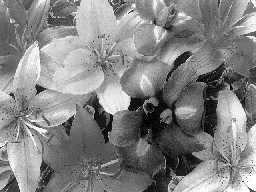
\includegraphics[width=0.9\textwidth]{./sampleimages/sample1.png}
    \caption{元画像}
\end{subfigure}
\hfill
\begin{subfigure}[b]{0.45\textwidth}
    \centering
    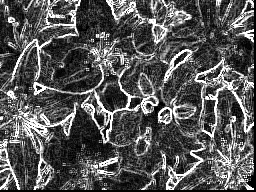
\includegraphics[width=0.9\textwidth]{./images/edge_enhanced_sample1_edge.png}
    \caption{エッジ強調}
\end{subfigure}

\begin{subfigure}[b]{0.45\textwidth}
    \centering
    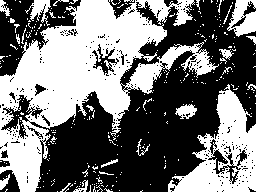
\includegraphics[width=0.9\textwidth]{./images/binarized_sample1_binary.png}
    \caption{二値化(閾値: 134)}
\end{subfigure}
\hfill
\begin{subfigure}[b]{0.45\textwidth}
    \centering
    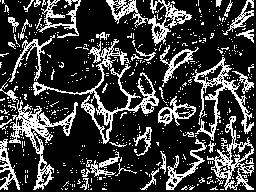
\includegraphics[width=0.9\textwidth]{./images/combined_sample1_combined.png}
    \caption{エッジ強調→二値化(閾値: 125)}
\end{subfigure}
\caption{sample1.pgm の処理結果}
\label{fig:sample1}
\end{figure}

\begin{figure}[!htbp]
\centering
\begin{subfigure}[b]{0.45\textwidth}
    \centering
    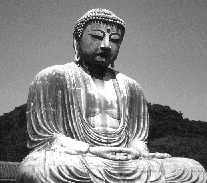
\includegraphics[width=0.9\textwidth]{./sampleimages/sample2.png}
    \caption{元画像}
\end{subfigure}
\hfill
\begin{subfigure}[b]{0.45\textwidth}
    \centering
    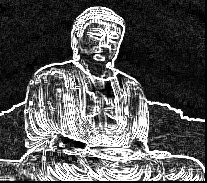
\includegraphics[width=0.9\textwidth]{./images/edge_enhanced_sample2_edge.png}
    \caption{エッジ強調}
\end{subfigure}

\begin{subfigure}[b]{0.45\textwidth}
    \centering
    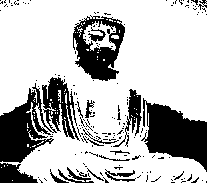
\includegraphics[width=0.9\textwidth]{./images/binarized_sample2_binary.png}
    \caption{二値化(閾値: 111)}
\end{subfigure}
\hfill
\begin{subfigure}[b]{0.45\textwidth}
    \centering
    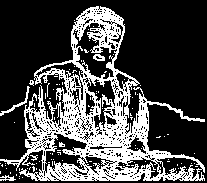
\includegraphics[width=0.9\textwidth]{./images/combined_sample2_combined.png}
    \caption{エッジ強調→二値化(閾値: 127)}
\end{subfigure}
\caption{sample2.pgm の処理結果}
\label{fig:sample2}
\end{figure}

\begin{figure}[!htbp]
\centering
\begin{subfigure}[b]{0.45\textwidth}
    \centering
    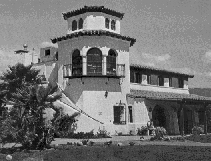
\includegraphics[width=0.9\textwidth]{./sampleimages/sample3.png}
    \caption{元画像}
\end{subfigure}
\hfill
\begin{subfigure}[b]{0.45\textwidth}
    \centering
    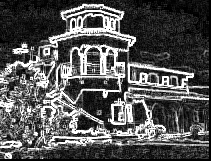
\includegraphics[width=0.9\textwidth]{./images/edge_enhanced_sample3_edge.png}
    \caption{エッジ強調}
\end{subfigure}

\begin{subfigure}[b]{0.45\textwidth}
    \centering
    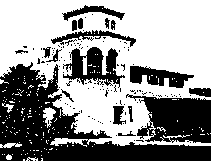
\includegraphics[width=0.9\textwidth]{./images/binarized_sample3_binary.png}
    \caption{二値化(閾値: 105)}
\end{subfigure}
\hfill
\begin{subfigure}[b]{0.45\textwidth}
    \centering
    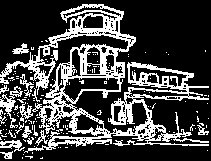
\includegraphics[width=0.9\textwidth]{./images/combined_sample3_combined.png}
    \caption{エッジ強調→二値化(閾値: 125)}
\end{subfigure}
\caption{sample3.pgm の処理結果}
\label{fig:sample3}
\end{figure}

\begin{figure}[!htbp]
\centering
\begin{subfigure}[b]{0.45\textwidth}
    \centering
    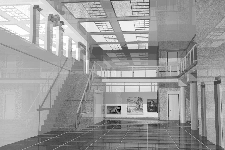
\includegraphics[width=0.9\textwidth]{./sampleimages/sample4.png}
    \caption{元画像}
\end{subfigure}
\hfill
\begin{subfigure}[b]{0.45\textwidth}
    \centering
    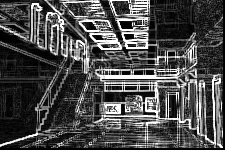
\includegraphics[width=0.9\textwidth]{./images/edge_enhanced_sample4_edge.png}
    \caption{エッジ強調}
\end{subfigure}

\begin{subfigure}[b]{0.45\textwidth}
    \centering
    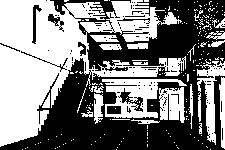
\includegraphics[width=0.9\textwidth]{./images/binarized_sample4_binary.png}
    \caption{二値化(閾値: 155)}
\end{subfigure}
\hfill
\begin{subfigure}[b]{0.45\textwidth}
    \centering
    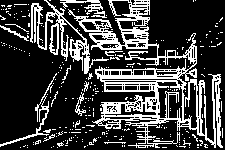
\includegraphics[width=0.9\textwidth]{./images/combined_sample4_combined.png}
    \caption{エッジ強調→二値化(閾値: 112)}
\end{subfigure}
\caption{sample4.pgm の処理結果}
\label{fig:sample4}
\end{figure}

\begin{figure}[!htbp]
\centering
\begin{subfigure}[b]{0.45\textwidth}
    \centering
    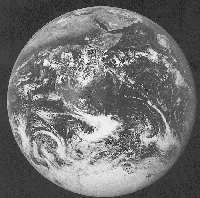
\includegraphics[width=0.9\textwidth]{./sampleimages/sample5.png}
    \caption{元画像}
\end{subfigure}
\hfill
\begin{subfigure}[b]{0.45\textwidth}
    \centering
    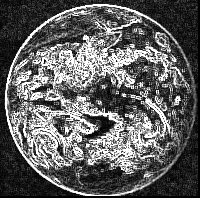
\includegraphics[width=0.9\textwidth]{./images/edge_enhanced_sample5_edge.png}
    \caption{エッジ強調}
\end{subfigure}

\begin{subfigure}[b]{0.45\textwidth}
    \centering
    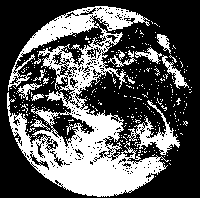
\includegraphics[width=0.9\textwidth]{./images/binarized_sample5_binary.png}
    \caption{二値化(閾値: 128)}
\end{subfigure}
\hfill
\begin{subfigure}[b]{0.45\textwidth}
    \centering
    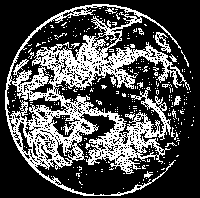
\includegraphics[width=0.9\textwidth]{./images/combined_sample5_combined.png}
    \caption{エッジ強調→二値化(閾値: 128)}
\end{subfigure}
\caption{sample5.pgm の処理結果}
\label{fig:sample5}
\end{figure}

\begin{figure}[!htbp]
\centering
\begin{subfigure}[b]{0.45\textwidth}
    \centering
    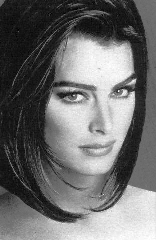
\includegraphics[width=0.9\textwidth]{./sampleimages/sample6.png}
    \caption{元画像}
\end{subfigure}
\hfill
\begin{subfigure}[b]{0.45\textwidth}
    \centering
    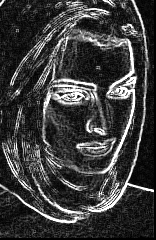
\includegraphics[width=0.9\textwidth]{./images/edge_enhanced_sample6_edge.png}
    \caption{エッジ強調}
\end{subfigure}

\begin{subfigure}[b]{0.45\textwidth}
    \centering
    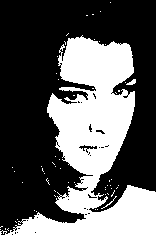
\includegraphics[width=0.9\textwidth]{./images/binarized_sample6_binary.png}
    \caption{二値化(閾値: 127)}
\end{subfigure}
\hfill
\begin{subfigure}[b]{0.45\textwidth}
    \centering
    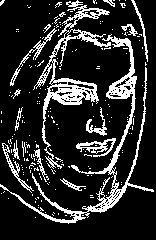
\includegraphics[width=0.9\textwidth]{./images/combined_sample6_combined.png}
    \caption{エッジ強調→二値化(閾値: 109)}
\end{subfigure}
\caption{sample6.pgm の処理結果}
\label{fig:sample6}
\end{figure}

\begin{figure}[!htbp]
\centering
\begin{subfigure}[b]{0.45\textwidth}
    \centering
    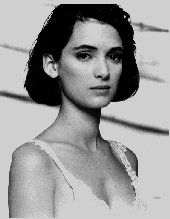
\includegraphics[width=0.9\textwidth]{./sampleimages/sample7.png}
    \caption{元画像}
\end{subfigure}
\hfill
\begin{subfigure}[b]{0.45\textwidth}
    \centering
    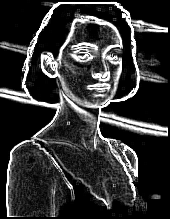
\includegraphics[width=0.9\textwidth]{./images/edge_enhanced_sample7_edge.png}
    \caption{エッジ強調}
\end{subfigure}

\begin{subfigure}[b]{0.45\textwidth}
    \centering
    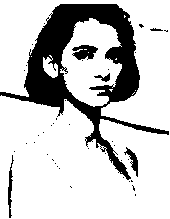
\includegraphics[width=0.9\textwidth]{./images/binarized_sample7_binary.png}
    \caption{二値化(閾値: 107)}
\end{subfigure}
\hfill
\begin{subfigure}[b]{0.45\textwidth}
    \centering
    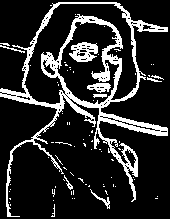
\includegraphics[width=0.9\textwidth]{./images/combined_sample7_combined.png}
    \caption{エッジ強調→二値化(閾値: 114)}
\end{subfigure}
\caption{sample7.pgm の処理結果}
\label{fig:sample7}
\end{figure}

\begin{figure}[!htbp]
\centering
\begin{subfigure}[b]{0.45\textwidth}
    \centering
    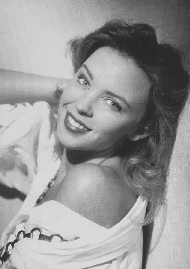
\includegraphics[width=0.9\textwidth]{./sampleimages/sample8.png}
    \caption{元画像}
\end{subfigure}
\hfill
\begin{subfigure}[b]{0.45\textwidth}
    \centering
    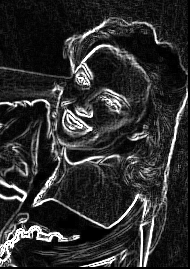
\includegraphics[width=0.9\textwidth]{./images/edge_enhanced_sample8_edge.png}
    \caption{エッジ強調}
\end{subfigure}

\begin{subfigure}[b]{0.45\textwidth}
    \centering
    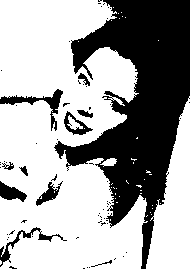
\includegraphics[width=0.9\textwidth]{./images/binarized_sample8_binary.png}
    \caption{二値化(閾値: 136)}
\end{subfigure}
\hfill
\begin{subfigure}[b]{0.45\textwidth}
    \centering
    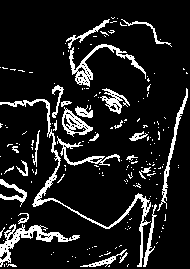
\includegraphics[width=0.9\textwidth]{./images/combined_sample8_combined.png}
    \caption{エッジ強調→二値化(閾値: 105)}
\end{subfigure}
\caption{sample8.pgm の処理結果}
\label{fig:sample8}
\end{figure}

\begin{figure}[!htbp]
\centering
\begin{subfigure}[b]{0.45\textwidth}
    \centering
    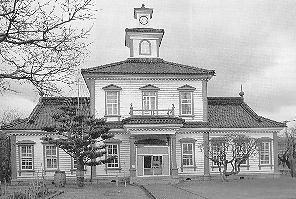
\includegraphics[width=0.9\textwidth]{./sampleimages/sample9.png}
    \caption{元画像}
\end{subfigure}
\hfill
\begin{subfigure}[b]{0.45\textwidth}
    \centering
    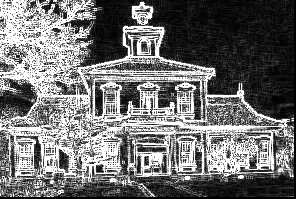
\includegraphics[width=0.9\textwidth]{./images/edge_enhanced_sample9_edge.png}
    \caption{エッジ強調}
\end{subfigure}

\begin{subfigure}[b]{0.45\textwidth}
    \centering
    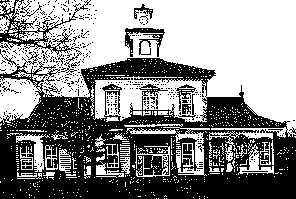
\includegraphics[width=0.9\textwidth]{./images/binarized_sample9_binary.png}
    \caption{二値化(閾値: 162)}
\end{subfigure}
\hfill
\begin{subfigure}[b]{0.45\textwidth}
    \centering
    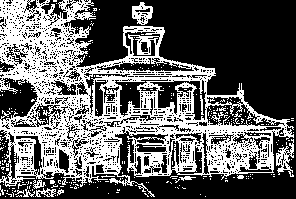
\includegraphics[width=0.9\textwidth]{./images/combined_sample9_combined.png}
    \caption{エッジ強調→二値化(閾値: 133)}
\end{subfigure}
\caption{sample9.pgm の処理結果}
\label{fig:sample9}
\end{figure}

\begin{figure}[!htbp]
\centering
\begin{subfigure}[b]{0.45\textwidth}
    \centering
    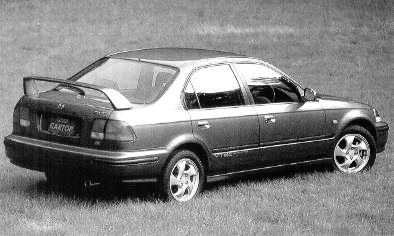
\includegraphics[width=0.9\textwidth]{./sampleimages/sample10.png}
    \caption{元画像}
\end{subfigure}
\hfill
\begin{subfigure}[b]{0.45\textwidth}
    \centering
    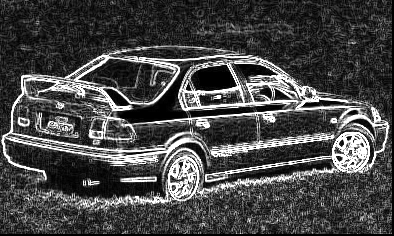
\includegraphics[width=0.9\textwidth]{./images/edge_enhanced_sample10_edge.png}
    \caption{エッジ強調}
\end{subfigure}

\begin{subfigure}[b]{0.45\textwidth}
    \centering
    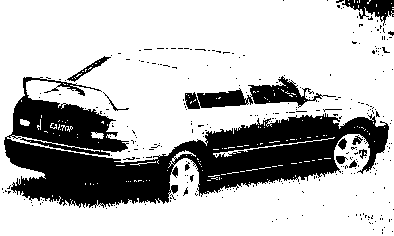
\includegraphics[width=0.9\textwidth]{./images/binarized_sample10_binary.png}
    \caption{二値化(閾値: 103)}
\end{subfigure}
\hfill
\begin{subfigure}[b]{0.45\textwidth}
    \centering
    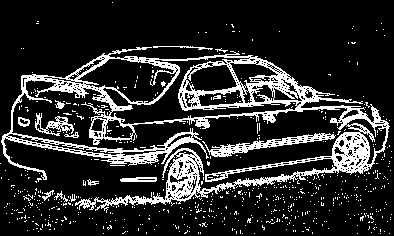
\includegraphics[width=0.9\textwidth]{./images/combined_sample10_combined.png}
    \caption{エッジ強調→二値化(閾値: 126)}
\end{subfigure}
\caption{sample10.pgm の処理結果}
\label{fig:sample10}
\end{figure}

\begin{figure}[!htbp]
\centering
\begin{subfigure}[b]{0.45\textwidth}
    \centering
    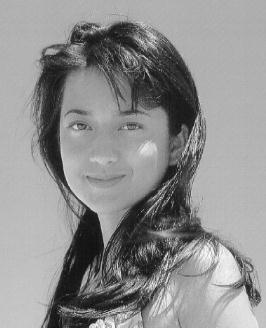
\includegraphics[width=0.9\textwidth]{./sampleimages/sample11.png}
    \caption{元画像}
\end{subfigure}
\hfill
\begin{subfigure}[b]{0.45\textwidth}
    \centering
    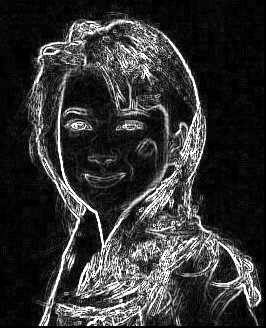
\includegraphics[width=0.9\textwidth]{./images/edge_enhanced_sample11_edge.png}
    \caption{エッジ強調}
\end{subfigure}

\begin{subfigure}[b]{0.45\textwidth}
    \centering
    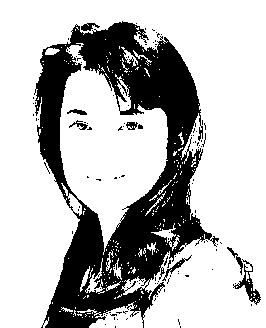
\includegraphics[width=0.9\textwidth]{./images/binarized_sample11_binary.png}
    \caption{二値化(閾値: 117)}
\end{subfigure}
\hfill
\begin{subfigure}[b]{0.45\textwidth}
    \centering
    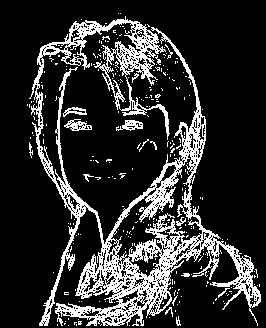
\includegraphics[width=0.9\textwidth]{./images/combined_sample11_combined.png}
    \caption{エッジ強調→二値化(閾値: 100)}
\end{subfigure}
\caption{sample11.pgm の処理結果}
\label{fig:sample11}
\end{figure}

\begin{figure}[!htbp]
\centering
\begin{subfigure}[b]{0.45\textwidth}
    \centering
    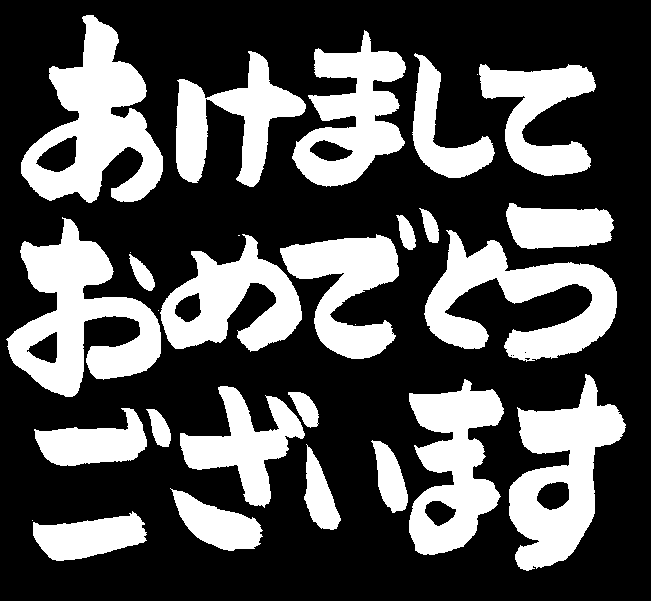
\includegraphics[width=0.9\textwidth]{./sampleimages/sample12.png}
    \caption{元画像}
\end{subfigure}
\hfill
\begin{subfigure}[b]{0.45\textwidth}
    \centering
    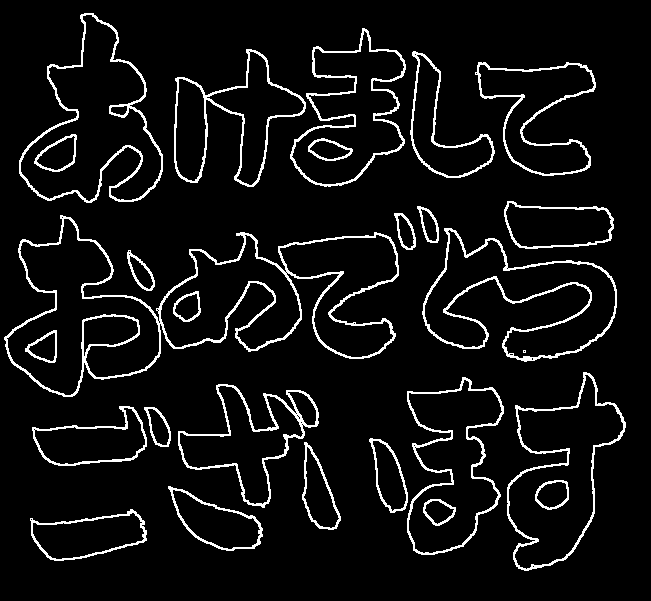
\includegraphics[width=0.9\textwidth]{./images/edge_enhanced_sample12_edge.png}
    \caption{エッジ強調}
\end{subfigure}

\begin{subfigure}[b]{0.45\textwidth}
    \centering
    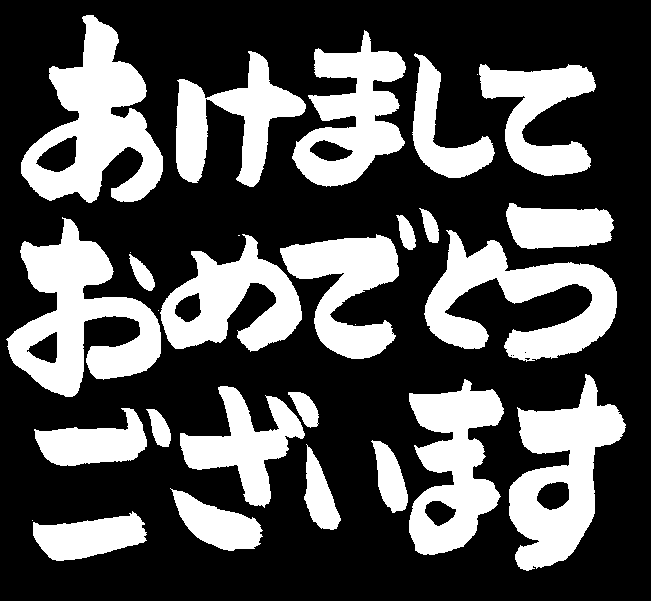
\includegraphics[width=0.9\textwidth]{./images/binarized_sample12_binary.png}
    \caption{二値化(閾値: 1)}
\end{subfigure}
\hfill
\begin{subfigure}[b]{0.45\textwidth}
    \centering
    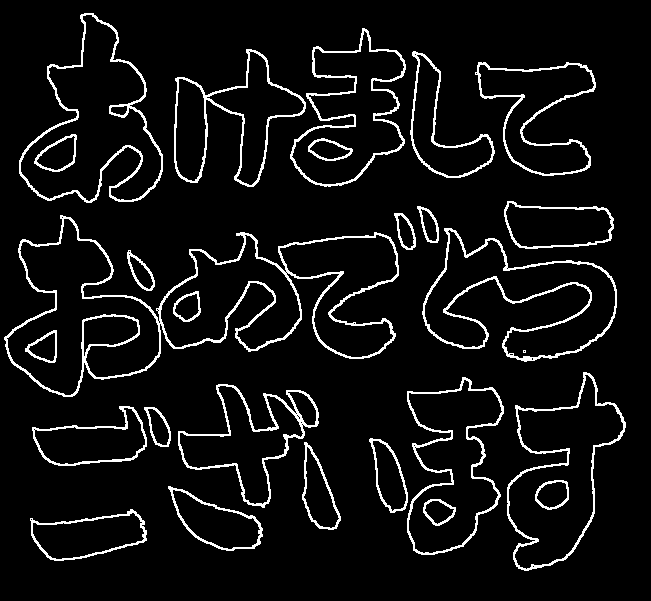
\includegraphics[width=0.9\textwidth]{./images/combined_sample12_combined.png}
    \caption{エッジ強調→二値化(閾値: 1)}
\end{subfigure}
\caption{sample12.pgm の処理結果}
\label{fig:sample12}
\end{figure}

\begin{figure}[!htbp]
\centering
\begin{subfigure}[b]{0.45\textwidth}
    \centering
    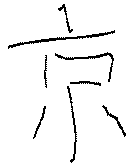
\includegraphics[width=0.9\textwidth]{./sampleimages/sample13.png}
    \caption{元画像}
\end{subfigure}
\hfill
\begin{subfigure}[b]{0.45\textwidth}
    \centering
    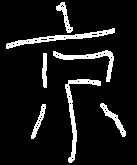
\includegraphics[width=0.9\textwidth]{./images/edge_enhanced_sample13_edge.png}
    \caption{エッジ強調}
\end{subfigure}

\begin{subfigure}[b]{0.45\textwidth}
    \centering
    \includegraphics[width=0.9\textwidth]{./images/binarized_sample13_binary.png}
    \caption{二値化(閾値: 1)}
\end{subfigure}
\hfill
\begin{subfigure}[b]{0.45\textwidth}
    \centering
    \includegraphics[width=0.9\textwidth]{./images/combined_sample13_combined.png}
    \caption{エッジ強調→二値化(閾値: 1)}
\end{subfigure}
\caption{sample13.pgm の処理結果}
\label{fig:sample13}
\end{figure}


\end{document}
